\documentclass{article}
\usepackage{graphicx}
\usepackage{verbatim}
\usepackage{amsmath}
\usepackage{listings}

\title{Code book}
\author{Aaron Nova, Till Nils Böhringer, \\ 
Moises De Jesus Maldonado Alonso, Florian Hellwig}
\date{23.05.2024}

\newcommand\Plotwidth{0.8}
\newcommand\Bilderwidth{0.8}

\begin{document}

\maketitle

\section{Datasets}

\subsection{Significant earthquake database (CSV): 1193 entries from 2000-2020}
\begin{itemize}
\item \textbf{Source:} National Centers for
Environmental Information
\item \textbf{Information about the dataset:} Contains data about time point, location, magnitude, financial costs and human losses of earthquakes which happened in the years 2000-2020
\item \textbf{Date of retrieval:} 18.04.2024
\item \textbf{Data Source:} https://www.ngdc.noaa.gov/hazel/view/hazards/earthquake/event-data?maxYear=2020\&minYear=1999
\end{itemize}

\begin{comment}

\subsection{WHICH ONE WILL WE USE? Population density of the world, years 2000, 2005, 2010, 2015, 2020 (GeoTIFF (.tif) and ASCII (.asc))}
\begin{itemize}
\item \textbf{Source:} [Insert Dataset Name]
\item \textbf{Information of the dataset:} [Insert information]
\item \textbf{Date of retrieval:} 
\item \textbf{Data Source:} https://sedac.ciesin.columbia.edu/data/set/gpw-v4-population-density-rev11/data-download
\end{itemize}

\subsection{WHICH ONE WILL WE USE? High-Resolution Population Density Maps around the year 2020 (GeoTIFF sometimes CSV)}
\begin{itemize}
\item \textbf{Source:} [Insert Dataset Name]
\item \textbf{Information of the dataset:} [Insert information]
\item \textbf{Date of retrieval:} [Insert Date]
\item \textbf{Data Source:} DOES NOT WORK: https://data.humdata.org/organization/meta?q=population%20density&sort=score%20desc%2C%2 
\end{itemize}

\end{comment}

\subsection{Average national income from 2000-2020 (CSV)}
\begin{itemize}
\item \textbf{Source:} World Inequality Database
\item \textbf{Information of the dataset:} Contains the average national income and the average income of the poorer half of the population for different countries for every year between 2000 and 2020
\item \textbf{Date of retrieval:} 23.04.2024
\item \textbf{Data Source:} https://wid.world/data/
\end{itemize}

\subsection{Population Counts / Unconstrained global mosaics 2000-2020 ( 1 km resolution )}
\begin{itemize}
\item \textbf{Source:} WorldPop Hub
\item \textbf{Information of the dataset:} Contains the population counts of the different parts of the world with a resolution of 1 $\text{km}^2$
\item \textbf{Date of retrieval:} 04.05.2024
\item \textbf{Data Source:} https://hub.worldpop.org/geodata/listing?id=64
\end{itemize}

\section{Variables in the cleaned Master Data frame}

\subsection{Year}
\begin{itemize}
    \item \textbf{Description:} Year the earthquake happened
    \item \textbf{Type:} Numerical
    \item \textbf{Units:} -
    \item \textbf{Range/Values:} 2000 - 2020, integers
    \item \textbf{Missing Values:} ??? How missing values were handled
    \item \textbf{Notes:} -
\end{itemize}

\begin{comment}
\subsection{Mo}
\begin{itemize}
    \item \textbf{Description:} Month the earthquake happened
    \item \textbf{Type:} Numerical
    \item \textbf{Units:} -
    \item \textbf{Range/Values:} 1 - 12, integers
    \item \textbf{Missing Values:} ???
    \item \textbf{Notes:} -
\end{itemize}

\subsection{Dy}
\begin{itemize}
    \item \textbf{Description:} Day the earthquake happened 
    \item \textbf{Type:} Numerical
    \item \textbf{Units:} -
    \item \textbf{Range/Values:} 1 - 31, integers
    \item \textbf{Missing Values:} ???
    \item \textbf{Notes:} -
\end{itemize}

\subsection{Hr}
\begin{itemize}
    \item \textbf{Description:} Hour the earthquake happened  
    \item \textbf{Type:} Numerical
    \item \textbf{Units:} -
    \item \textbf{Range/Values:} 0 - 23, integers (but displayed as floating point numbers)
    \item \textbf{Missing Values:} ???
    \item \textbf{Notes:} -
\end{itemize}

\end{comment}

\begin{comment}

\subsection{Mn}
\begin{itemize}
    \item \textbf{Description:} Minute the earthquake happened  
    \item \textbf{Type:} Numerical
    \item \textbf{Units:} -
    \item \textbf{Range/Values:} 0 - 59, integers (but displayed as floating point numbers)
    \item \textbf{Missing Values:} ???
    \item \textbf{Notes:} -
\end{itemize}

\subsection{Sec}
\begin{itemize}
    \item \textbf{Description:} Second the earthquake happened  
    \item \textbf{Type:} Numerical
    \item \textbf{Units:} -
    \item \textbf{Range/Values:} 0.0 - 59.9, rounded to the nearest tenth
    \item \textbf{Missing Values:} ???
    \item \textbf{Notes:} -
\end{itemize}

\subsection{Tsu}
\begin{itemize}
    \item \textbf{Description:} ??? 
    \item \textbf{Type:} ???
    \item \textbf{Units:} ???
    \item \textbf{Range/Values:} ???
    \item \textbf{Missing Values:} ???
    \item \textbf{Notes:} ???
\end{itemize}

\subsection{Vol}
\begin{itemize}
    \item \textbf{Description:} ??? 
    \item \textbf{Type:} ???
    \item \textbf{Units:} ???
    \item \textbf{Range/Values:} ???
    \item \textbf{Missing Values:} ???
    \item \textbf{Notes:} ???
\end{itemize}

\end{comment}

\subsection{Country}
\begin{itemize}
    \item \textbf{Description:} Country where the earthquake happened
    \item \textbf{Type:} Categorical
    \item \textbf{Units:} -
    \item \textbf{Range/Values:} Countries worldwide
    \item \textbf{Missing Values:} ???
    \item \textbf{Notes:} -
\end{itemize}

\begin{comment}

\subsection{Location Name}
\begin{itemize}
    \item \textbf{Description:} Location where the earthquake happened (with country and location name)
    \item \textbf{Type:} String ???
    \item \textbf{Units:} -
    \item \textbf{Range/Values:} -
    \item \textbf{Missing Values:} ???
    \item \textbf{Notes:} -
\end{itemize}

\end{comment}

\begin{comment}

\subsection{Region}
\begin{itemize}
    \item \textbf{Description:} Region where the earthquake happened
    \item \textbf{Type:} Categorical
    \item \textbf{Units:} -
    \item \textbf{Range/Values:} Regions worldwide
    \item \textbf{Missing Values:} ???
    \item \textbf{Notes:} -
\end{itemize}

\end{comment}

\subsection{Latitude}
\begin{itemize}
    \item \textbf{Description:} Latitude of the location where the earthquake happened
    \item \textbf{Type:} Numerical
    \item \textbf{Units:} Degrees
    \item \textbf{Range/Values:} -90 - 90, rounded to the nearest thousandths
    \item \textbf{Missing Values:} ???
    \item \textbf{Notes:} -
\end{itemize}

\subsection{Longitude}
\begin{itemize}
    \item \textbf{Description:} Longitude of the location where the earthquake happened
    \item \textbf{Type:} Numerical
    \item \textbf{Units:} Degrees
    \item \textbf{Range/Values:} -180 - 180, rounded to the nearest thousandths
    \item \textbf{Missing Values:} ???
    \item \textbf{Notes:} -
\end{itemize}

\subsection{Focal Depth (km)}
\begin{itemize}
    \item \textbf{Description:} Focal depth of the earthquake
    \item \textbf{Type:} Numerical
    \item \textbf{Units:} Kilometers
    \item \textbf{Range/Values:} Positive integers
    \item \textbf{Missing Values:} ???
    \item \textbf{Notes:} -
\end{itemize}

\subsection{Mag}
\begin{itemize}
    \item \textbf{Description:} Magnitude of the earthquake on the richter scale
    \item \textbf{Type:} Numerical
    \item \textbf{Units:} -
    \item \textbf{Range/Values:} ??? (depends on the scale)
    \item \textbf{Missing Values:} ???
    \item \textbf{Notes:} -
\end{itemize}

\subsection{Average Income}
\begin{itemize}
    \item \textbf{Description:} Average yearly income of the population of the country where the earthquake happened
    \item \textbf{Type:} Numerical
    \item \textbf{Units:} US-Dollars
    \item \textbf{Range/Values:} Positive values, rounded to the next ten thousandth
    \item \textbf{Missing Values:} ???
    \item \textbf{Notes:} -
\end{itemize}

\subsection{p0p50\_share}
\begin{itemize}
    \item \textbf{Description:} Percentage of the total income of the poorer half of the population compared to the total income of the whole population
    \item \textbf{Type:} Numerical
    \item \textbf{Units:} Percentage
    \item \textbf{Range/Values:} Between 0 and 1, rounded to the next ten thousandth
    \item \textbf{Missing Values:} ???
    \item \textbf{Notes:} -
\end{itemize}

\subsection{pop\_total}
\begin{itemize}
    \item \textbf{Description:} Total Population in preperation Radius
    \item \textbf{Type:} Numerical
    \item \textbf{Units:} -
    \item \textbf{Range/Values:} Positive floats, rounded to neares integer
    \item \textbf{Missing Values:} -
    \item \textbf{Notes:} The total population got calculated with the population density data. With the magnitude, the preperation radius got calculated and then all people within this radius summed up. This happends in the File \lstinline{"pop_regional.ipynb"}
\end{itemize}

\subsection{Total Deaths}
\begin{itemize}
    \item \textbf{Description:} Number of deaths because of the earthquake
    \item \textbf{Type:} Numerical
    \item \textbf{Units:} People
    \item \textbf{Range/Values:} Non negative integers
    \item \textbf{Missing Values:} ???
    \item \textbf{Notes:} -
\end{itemize}

\subsection{Total Injuries}
\begin{itemize}
    \item \textbf{Description:} Number of people injured because of the earthquake
    \item \textbf{Type:} Numerical
    \item \textbf{Units:} People
    \item \textbf{Range/Values:} Non negative integers
    \item \textbf{Missing Values:} ???
    \item \textbf{Notes:} -
\end{itemize}

\subsection{Total Damage (\$Mil)}
\begin{itemize}
    \item \textbf{Description:} Total financial damage the earthquake has caused
    \item \textbf{Type:} Numerical
    \item \textbf{Units:} Millions US-Dollars
    \item \textbf{Range/Values:} Non negative values 
    \item \textbf{Missing Values:} ???
    \item \textbf{Notes:} -
\end{itemize}


\subsection{Total Houses Destroyed}
\begin{itemize}
    \item \textbf{Description:} Number of houses destroyed because of the earthquake
    \item \textbf{Type:} Numerical
    \item \textbf{Units:} Houses
    \item \textbf{Range/Values:} Non negative integers
    \item \textbf{Missing Values:} ???
    \item \textbf{Notes:} -
\end{itemize}

\subsection{Total Houses Damaged}
\begin{itemize}
    \item \textbf{Description:} Number of houses damaged because of the earthquake
    \item \textbf{Type:} Numerical
    \item \textbf{Units:} Houses
    \item \textbf{Range/Values:} Non negative integers
    \item \textbf{Missing Values:} ???
    \item \textbf{Notes:} -
\end{itemize}

\subsection{Total Death Description}
\begin{itemize}
    \item \textbf{Description:} Classification of the strength of the earthquake based on the number of deaths
    \item \textbf{Type:} Categorical
    \item \textbf{Units:} -
    \item \textbf{Range/Values:} $\{0,1,2,3,4 \}$
    \item \textbf{Missing Values:} Set to 0, based on the raw data it's assumed that if there were no deaths the field was left blank.
    \item \textbf{Notes:} 0: No deaths, 1: 1-50 deaths, 2: 51-100 deaths, 3: 101-1000 deaths, 4: more than 1000 deaths
\end{itemize}

\subsection{Total Injuries Description}
\begin{itemize}
    \item \textbf{Description:} Classification of the strength of the earthquake based on the number of people injured
    \item \textbf{Type:} Categorical
    \item \textbf{Units:} -
    \item \textbf{Range/Values:} $\{0,1,2,3,4 \}$
    \item \textbf{Missing Values:} Set to 0, based on the raw data it's assumed that if there were no injuries the field was left blank.
    \item \textbf{Notes:} 0: No people injured, 1: 1-50 people injured, 2: 51-100 people injured, 3: 101-1000 people injured, 4: more than 1000 people injured
\end{itemize}

\subsection{Total Damage Description}
\begin{itemize}
    \item \textbf{Description:} Classification of the strength of the earthquake based on the total financial damage
    \item \textbf{Type:} Categorical
    \item \textbf{Units:} -
    \item \textbf{Range/Values:} $\{0,1,2,3,4 \}$
    \item \textbf{Missing Values:} Set to 0, based on the raw data it's assumed that if there were no damages the field was left blank.
    \item \textbf{Notes:} 0: No costs, 1: 0-1 million US-Dollars, 2: 1-5 million US-Dollars, 3: 5-30 million US-Dollars, 4: more than 30 million US-Dollars
\end{itemize}

\subsection{Total Houses Destroyed Description}
\begin{itemize}
    \item \textbf{Description:} Classification of the strength of the earthquake based on the number of houses destroyed
    \item \textbf{Type:} Categorical
    \item \textbf{Units:} -
    \item \textbf{Range/Values:} $\{0,1,2,3,4 \}$
    \item \textbf{Missing Values:} Set to 0, based on the raw data it's assumed that if there were no destroyed houses the field was left blank.
    \item \textbf{Notes:} 0: No houses destroyed, 1: 1-50 houses destroyed, 2: 51-100 houses destroyed, 3: 101-1000 houses destroyed, 4: more than 1000 houses destroyed
\end{itemize}

\subsection{Total Houses Damaged Description}
\begin{itemize}
    \item \textbf{Description:} Classification of the strength of the earthquake based on the number of houses damaged
    \item \textbf{Type:} Categorical
    \item \textbf{Units:} -
    \item \textbf{Range/Values:} $\{0,1,2,3,4 \}$
    \item \textbf{Missing Values:} Set to 0, based on the raw data it's assumed that if there were no damaged houses the field was left blank.
    \item \textbf{Notes:} 0: No houses damaged, 1: 1-50 houses damaged, 2: 51-100 houses damaged, 3: 101-1000 houses damaged, 4: more than 1000 houses damaged
\end{itemize}

\section{Summary choices}

\section{Study design}

\subsection{Dimension reduction}

The data is sparse, to combat this, the dimension of the data gets reduced. For the reduction, the description columns were chosen. These columns are already binned with adequate ranges, which speeds thing up. For the dimension reduction, PCA was considered. With the PCA, it's not clear how the data columns are calculated together, and it's also not clear that a lower value after the PCA is necessarily a low value for all included columns. Therefore, a second choice was made to sum all columns and then map the values between 0 and 1. Because the columns are all already all between 0 and 4 there don't need to be normalised.

\begin{figure}[h]
    \centering
    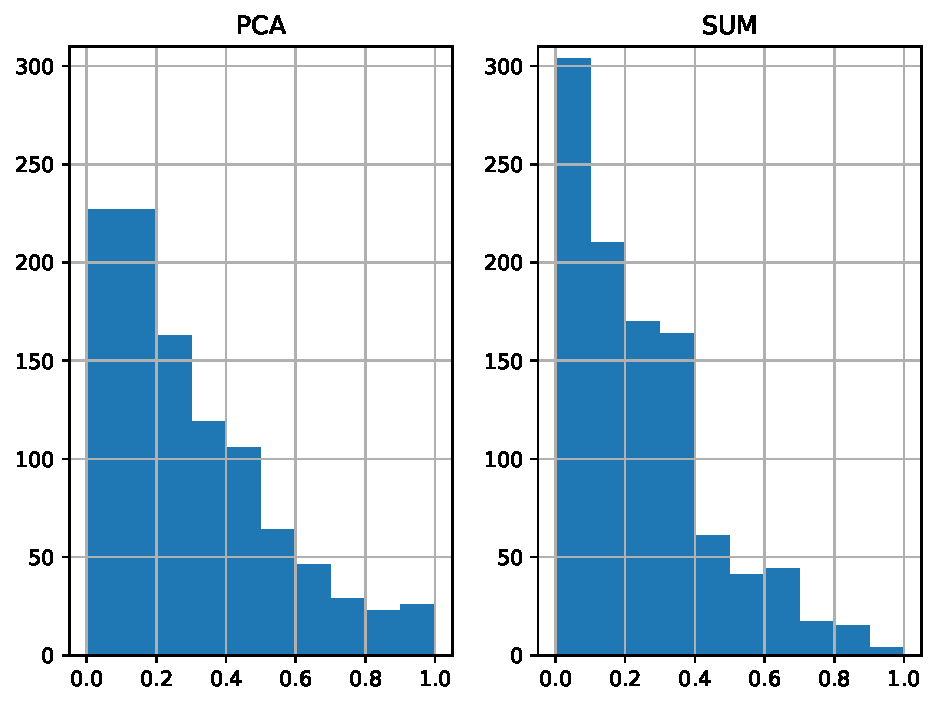
\includegraphics[width=\Plotwidth\textwidth]{Plots/PCA_SUM.pdf}
    \caption{Comparison between PCA and SUM over the reduced columns.}
    \label{fig:PCA_SUM}
\end{figure}

In figure \ref{fig:PCA_SUM} can be seen, the Histograms between PCA and SUM are fairly similar. This is all in the file \lstinline{"dimension_reduction.ipynb"}

\end{document}
